\documentclass{article}
\usepackage{graphicx}
\usepackage{fixmath}
\usepackage{gensymb}
\usepackage{listings}
\usepackage[margin=1in]{geometry}
\usepackage{multicol}
\usepackage{subfigure}


\begin{document}

\title{Literature Review}
\author{Romeo Orsolino}

\maketitle
\tableofcontents
\begin{abstract}
This is a collection of the literature review of my PhD. I wrote a small summary for each paper I read and I consider interesting for the topic of dynamic locomotion.
\end{abstract}
\section{Raibert - Running on four legs as though they were one -1986}

\subsection*{Summary}

In this paper the concept of \textbf{Virtual leg} is introduced. A virtual leg is a fictitious leg which mirrors the result of the locomotion performed by two or more legs which are in the same time on the ground.

\subsection*{Take aways}

\begin{itemize}
\item The control scheme implemented in this work, as much as Raibert's preceeding work on the one-legged hopper, is based on the idea to decouple the three main quantities of interest for locomotion: the robot's \textbf{pitch} angle, the \textbf{forward speed} and the \textbf{height} of each single jump.

\item The forward velocity and step lenght are adjusted making use of the so called \textbf{neutral point}, which is the point on the ground that, if the foothold is placed in that very same point, produces a constant speed (neither acceleration nor deceleration)

\item \textbf{One-foot gaits} are defined as those gaits which can be performed with the use of one single virtual leg. These gaits can be performed theoretically with any number of legs, but they must all be coordinated in such a way to obtain the behavior of one single leg.
\end{itemize}
\section{Raibert - Adjusting step lenght for rough terrain locomotion - 1991}
\section{McGeer - Passive Dynamic Walking - 1990}
\section{Kalakrishnan, Buchli, Mistry, Schaal - Learning, Planning and control for quadruped locomotion over challenging terrain}
\section{Modeling and Control of Legged Robots \cite{Tedrake1}}
Authors: Wieber, Tedrake, Kuindersma\\
Year: 2015\\
\subsection*{Summary}
This documents develops a comprehensive summary regarding the main tools available to design dynamic gaits for walking robots (biped robots specifically). A particular focus is given to the controllability of the gait and the robustness analysis; the following four stability measures are explained:
\begin{itemize}
\item Robust stability
\item Stochastic stability
\item Input-Output stability
\item Stability margin: keeping away from boundaries such as the distance between the CoP and the edge of the convex support polygon.
\end{itemize}
The control design has got the following main tools for the robustness analysis of a given gait:
\begin{itemize}
\item Fixed points: A fixed point is a safe configuration of the robot where it can stand still;
\item Limit cycles: it represents an extension of the fixed point to the case of periodic gaits. More precisely it is a periodic orbit, namely a solution $\{q(t), u(t), f(t) | t \in [0,\infty) \}$ such that $q(t+T) = q(t)$, $u(t+T) = u(t)$ and $f(t+T) = f(t)$ where T is the period of the periodic orbit in the phase plane. A periodic solution is (asymptotically) orbitally stable if:
$$ \lim_{t\to\infty} [ \min_{0\leq t' \leq T} || q(t) - q_0(t')|| ] = 0$$
This means that the trajectories must not converge, only the distance between the initial point and the closest point must go to zero. This can be defined in a region containing $q_0(.)$ or globally (even if globally stable legged robots are of little interest).
The existence of such limit cycle depends on the actuation of the system, for a highly underactuated (or even passive) robot the computation of a limit cycle can be very challenging. As an opposite, for fully actuated robots, there exist many control policies $\mathbf{u}(t) = \mathbold{\pi} (t, \mathbf{q}(t),\dot{\mathbf{q}}(t),\mathbf{f}(t)$ that will lead to a limit cycle.
\item Viability = viability is referred to as ''not falling down'' capability. The viable space is thus defined as the set of states where the robot is able to avoid to fall down.
\item Controllability = capability to bring the robot from an arbitrary initial state to a final one within a finite time. In linear systems this is a property of the system, regardless of the initial and final conditions and it can be analysed by means of the controllability matrix. For nonlinear systems instead controllability is strongly dependent the initial and final states.
As a consequence we can distinguish different types of controllability depending on the initial and final states. For legged robots the controllability is considered as the ability to bring the system to a stable fixed point (called \textbf{capture point}). The set of initial states that can lead to a fixed point within a limited number of steps is called \textbf{capturable}. 
\end{itemize}



\subsection*{Key points / Takeaways}
\begin{enumerate}
\item definition of the Capture Point CP as a stable fixed point of the Poincaré Map
\item Clear description of the coupled dynamics of CoM, ZMP and CP.
\end{enumerate}
\subsection*{Weak points}
\subsection*{Ideas}
\begin{enumerate}
\item They should be better highlighted and fully described the links between CP and poincaré maps
\item Possibly the concept of CP should be extended to the ability to pass from a limit cycle to another limit cycle.
\item Worst case analysis of controller robustness has been given little attention so far. An extension of the Lyapunov functions-based methods shows that ''nominal solutions of the limit cycle are often parameter dependent''.
\end{enumerate}

\section{Tedrake - Underactuated Robotics}
\section{Tedrake - Bounding on rough terrain with the LittleDog Robot - 2011}
\section*{Summary}
\section{Wensing, Orin - High-speed humanoid running through control with a 3D-SLIP model}


\subsection*{Summary}
\section{J. Pratt, Goswami - Capture Point: A Step toward Humanoid Push Recovery \cite{Pratt+CDG:2006}}
Authors: J. Pratt, Goswami\\
Year: 2006
\subsection*{Summary}
The Capture Point CP is defined for push recovery purposes, namely for determining how many steps must be performed by the biped robot to recover from a push. This is done on a simplified LIP +  Flywheel model as the whole body dynamics of a robot is too complicated (being it highly dimensional, nonlinear and \textbf{hybrid}). First of all the CP is computed using the LIP model only, so that the robot can only act on the linear force $f_k$ for the push recovery, this leads to a unique point CP. The addition of the Flywheel acts as a further degree of freedom of the simplified model, that can use both $f_k$ and $\tau$ to recover from the push. This leads to the computation of a \textbf{capture region}, namely the set of all the capture points.
\begin{figure}
  \centering
  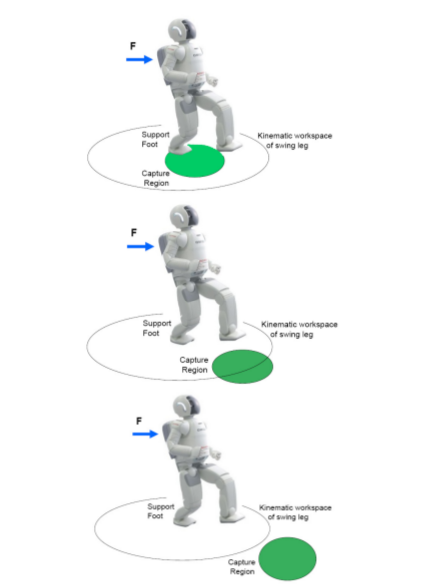
\includegraphics[width=90mm]{CapturePoint}
  \caption{The biped can recover from a push when its support polygon intersects the capture region}
\end{figure}
The different capture regions are computed for the following cases:
\begin{itemize}
\item Pure LIP model
\item LIP+Flywheel with instantaneous velocity variation
\item LIP+Flywheel with instantaneous position variation
\item LIP+Flywheel with limited torque and angle
\end{itemize}
\begin{figure}
  \centering
  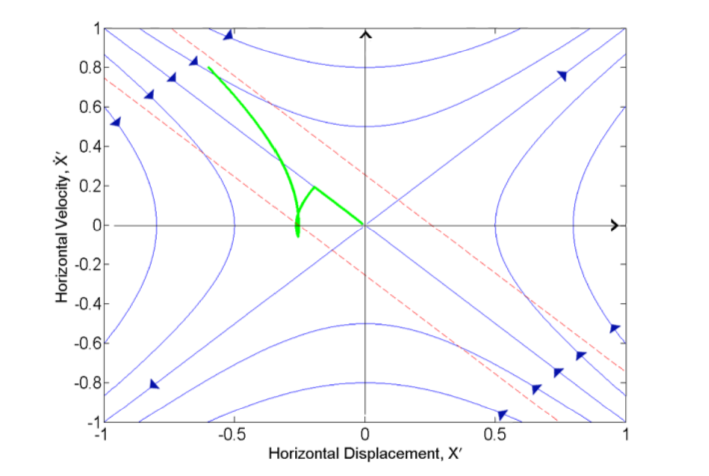
\includegraphics[width=90mm]{CPPhasePlane}
  \caption{Phase portrait of the LIP + Flywheel model}
  \label{PhasePlane}
\end{figure}
In figure \ref{PhasePlane} you can see here the trajectory of the x coordinate of the CoM starting from an arbitrary point and reaching a \textit{capture state} performing a \textit{safe feasible trajectory}. In the same figure also the capture region is represented with the red dotted line. You can see here that the green trajectory goes out of the capture region for a few instants, this is because the LIP+Flywheel as a non-null momentum in that points whereas the displayed capture region was computed for an initial state with null momentum.
\subsection*{Key points / Takeaways}
\begin{enumerate}
\item Closed-form expression of the CP for a LIP +  Flywheel model model 
\item Determining which is the best lunge profile to recover from the push, solving for example an optimization problem
\item The analysis of the capture region is carried out also with non-dimensional variables in order to detect the minimum number of variables needed.
\end{enumerate}
\subsection*{Weak points}
\begin{itemize}
\item What do the blue curves in the phase plane of figure \ref{PhasePlane} represent?
\end{itemize}
\subsection*{Ideas}
\begin{enumerate}
\item The definition of CP could be studied also for a SPRINGED LIP + Flywheel
\item How does the Phase Plane look like if we use the $(\dot{x},\ddot{x})$ variables? can we maybe in this case define a limit cycle and use the Poincaré return map for checking the system stability?
\end{enumerate}

\section{J. Pratt, Goswami - Capturability Based Analysis and Control of Legged Robots - Part 1 \cite{Koolen:2012:CAC:2344876.2344877} - 2011}
Authors: J. Pratt, Goswami\\
Year: 2012
\subsection*{Summary}
The Capture point theory is here explained for 3D-LIP model and for the 3D-LIPM model (with non zero moment of inertia)
The \textit{capturability} is updated at the end of every stance phase: there is no way to change the capturability during the swing phase.
\begin{figure}[h!]
\begin{subfigure}
  \centering
  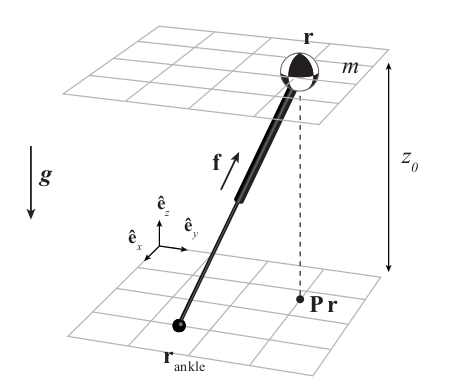
\includegraphics[width=50mm]{CP.png}
  \label{PhasePlane}
\end{subfigure}
\begin{subfigure}
  \centering
  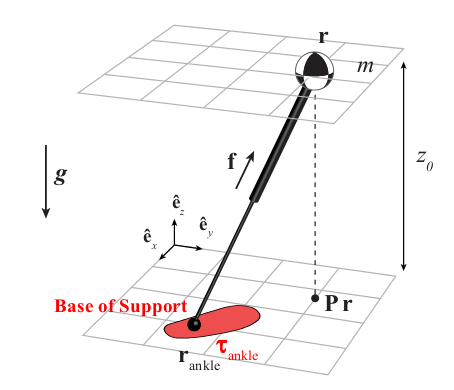
\includegraphics[width=50mm]{CPF.png}
  \label{PhasePlane}
\end{subfigure}
\begin{subfigure}
  \centering
  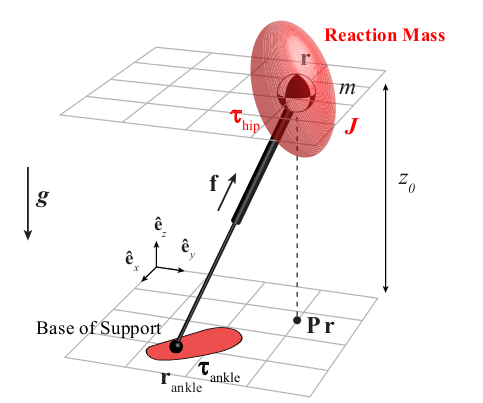
\includegraphics[width=50mm]{CPFM.png}
  \label{PhasePlane}
\end{subfigure}
\caption{three simplified models of a the dynamics of an antropomorphic robot}
\end{figure}
\begin{multicols}{3}
3D-LIP model:
\begin{enumerate}
\item Equations of motion:
$$ m \ddot{r} = mg + f $$
$$ -(r-r_{ankle})  \times f = 0 $$
\item CP definition:  $$ r_{ic} = P r + \frac{\dot{r}}{\omega} $$
\item Instantaneous CP dynamics: $$ \ddot{r} = \omega^2 (P r - r_{ankle}) $$
\item 0-step capturability:
$$ | r'_{ic} - r'_{ankle}| \le d'_0 = 0 $$
\item n-steps capturability:
$$ | r'_{ic} - r'_{ankle}| \le d'_n $$ where: $$ d'_n = (l'_{max} + d'_{n-1})e^{- \Delta t'_s}$$
\end{enumerate}
\columnbreak
3D-LIP + finite foot:
\begin{enumerate}
\item Equations of motion:
$$ m \ddot{r} = mg + f $$
$$ -(r-r_{ankle})  \times f + \tau_{ankle}= 0 $$
\item CP definition: \\
no c.f. sol.
\item Instantaneous CP dynamics:
$$ \ddot{r} = \omega^2 (P r - r_{CoP}) $$
\item 0-step capturability:
$$ | r'_{ic} - r'_{ankle}| \le d'_0 =  r'_{max} $$
\item n-steps capturability:
$$ | r'_{ic} - r'_{ankle}| \le d'_n $$ where: $ d'_n = r'_{max} + (l'_{max} - r'_{max} + d'_{n-1})e^{- \Delta t'_s}$
\end{enumerate}

\columnbreak
3D-LIP + finite foot + reaction mass:
\begin{enumerate}
\item Equations of motion:
$$ m \ddot{r} = mg + f $$
$$ J \dot{\omega} = \tau_{hip} - \omega \times (J \omega) $$
$$ -(r-r_{ankle})  \times f + \tau_{ankle} - \tau_{hip}= 0 $$
\item CP definition: 
no c.f. sol.
\item Instantaneous CP dynamics: $$ \ddot{r} = \omega^2 (P r - r_{CMP}) $$
$$ \dot{\omega} = J^{-1} P \tau_{hip} $$
\item 0-step capturability:
$$ | r'_{ic} - r'_{ankle}| \le d'_0 = r'_{max} + |\Delta r'_{CMP}|_{max}$$
\item n-steps capturability:
$$ | r'_{ic} - r'_{ankle}| \le d'_n $$ where: $ d'_n = r'_{max} + |\Delta r'_{CMP}|_{max} + (l'_{max} - r'_{max} + d'_{n-1})e^{- \Delta t'_s}$
\end{enumerate}
\end{multicols}
where:
\begin{itemize}
\item $P$ is the matrix which projects the CoM on the ground.
\item $r_{max}$ = distance between the CoP and the point on the edge of the support which is closest to the istantaneous CP.
\item CMP = Centroidal Moment Pivot point
\item $d_{\infty}$ = distance to the $\infty$-steps capturability region. This can be used as a \textbf{capturability margin}, in the sense that if the $d_{\infty}$ takes on a small value, the robot will likely fall when subject to an external disturbance. For example, using the same common parameters it was obtained that for:
\begin{itemize}
\item 3D-LIP model: $d_{\infty} = 0.431$
\item 3D-LIP model + finite foot: $d_{\infty} = 0.631$
\item 3D-LIP model + finite foot + reaction mass: $d_{\infty} = 0.664$
\end{itemize}
So we can conclude that the third model has got the \textit{highest level of capturability}, i.e. it is the most stable (see figure \ref{InftyCap}).
\\
\begin{figure}
  \centering
  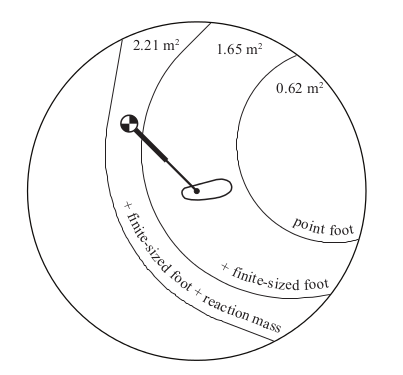
\includegraphics[width=50mm]{InftyCapturability.png}
  \caption{Comparison of the infinity-capturability distance $d_{\infty}$ for the three different considered models}
  \label{InftyCap}
\end{figure}
\end{itemize}
\subsection*{Key points / Takeaways}
\begin{itemize}
\item \textbf{Equivalent constant CoP} =
\end{itemize}
\subsection*{Weak points}
\subsection*{Ideas}


\section{J. Pratt, Goswami - Capturability Based Analysis and Control of Legged Robots - Part 2 \cite{Koolen:2012:CAC:2344876.2344877}}
Authors: J. Pratt, Goswami\\
Year: 2012
\subsection*{Summary}
The \textit{capturability} is updated at the end of every stance phase: there is no way to change the capturability during the swing phase.

\subsection*{Key points / Takeaways}
\subsection*{Weak points}
\subsection*{Ideas}


\section{Park, Kim - Quadruped Bounding Control with Variable Duty Cycle via Vertical Impulse Scaling - 2014}


\subsection*{Summary}
The strategy used by Park et al. consists in predefinig a given GRF profile parametrized by two Bezier curves. The overall force profile is normalized in such a way that the total energy given to the system in one stance period is equal to the work carried out by gravity during the flight phase $T$.
The relation is thus:

\begin{equation}
2 \alpha c T_{stance} = m g T
\end{equation}
where:
\begin{itemize}
\item c = normalizing factor
\item $\alpha$ = scaling factor
\end{itemize}
This model is completely stiff and the stance time decreases with the incrementation of the forward speed. The forward and vertical speeds are considered as decoupled though.\\
The next step consists in finding stable limit cycles; this is done by mean of the Poincarè Map: the system is linearized around a huge number of fixed points (varying both the Duty cycle and the stiffness of the PD controller) and the largest eigenvalue for each combination is plotted in a graph. In this graph only those eigenvalues which are smaller than 1 are considered as a stable solution. The final choice is made for the values of Duty cycle and stiffness which ensure the largest stability margin.
\begin{figure}[h]
  \centering
  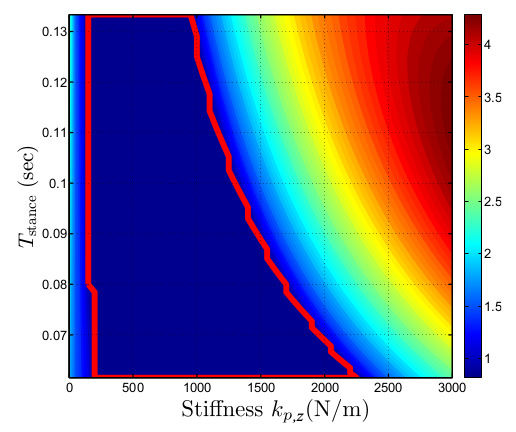
\includegraphics[width=100mm]{PoincarèMap.png}
  \caption{Poincarè Map to evaluate a stable solution}
  \label{InftyCap}
\end{figure}
\subsection*{Key Points / Takeaways}
\begin{itemize}
\item assumed values:
\begin{itemize}
\item $T_{swing} = 220$ ms;
\item $T_{air} = 43.5$ ms;
\item $T_{stance} = 66:133$ ms;
\item $T = T_{stance} + T_{swing}$
\item Duty cycle $D = 0.223:0.377$
\end{itemize}
\item horizontal and vertical speeds are considered as decoupled
\end{itemize}


\subsection*{Weak Points}

\begin{itemize}
\item In this paper there is no consideration of the landing and take off angle of the legs (angle of attack/"incidenza"). The GRF are computed using the trunk model only and massless legs. Therefore the dynamics of the legs is ignored and the compliance is not exploited.
\end{itemize}
\subsection*{Ideas} 
\begin{enumerate}
\item What about minimizing the stiffness of the SLIP model is such a way to damp the force peaks as much as possible??
\end{enumerate}

\section{Park - Quadrupedal galloping control for a wide range of speed via vertical impulse scaling - 2015}

\subsection*{Summary}
The baseline gait design is made of three optimization processes made in a cascade:
\begin{enumerate}
\item Optimization of the parameters associated to the ground reaction forces (decision variables are $\alpha^{GRF}_z$, $\alpha^{GRF}_x$ and $s$ (phase shift))
\item Design of the swing phase
\item Optimization process for obtaining the periodic limit cycle depending on the current speed (decision variables are stance time and swing time)
\end{enumerate}
\section{Park - Online Planning for Autonomous Running Jumps
Over Obstacles in High-Speed Quadrupeds \cite{Wensing2015} - 2015}
\section{D.E. Koditscheck - Sequential Composition of Dynamically Dexterous Robot Behaviors}
Authors: D.E. Koditschek\\
Year: 2015
\subsection*{Summary}
\begin{itemize}
\item Preimage backchaining concept is defined as inspired by [Lozano-Perez,Mason,Taylor 1984].
\item In this paper a clear approach to the problem of hybrid systems is given. An hybrid control problem is here defined as the problem of defining a control for a mix of continuous and discrete systems.
\item The coupled robot-environment state must be considered, not just one.
\item ''Event driven'' trajectory generators are needed.
\item The concept of invariant ellipsoid is given as the ellipsoid in the phase plane where the ball can be safely sent and there it does not lead to failure
\item Basically three different controllers are defined: juggling, catching and palming. Each of them is defined on a different sub-domain and a passage from one to another is made possible just thanks to a higher-level controller which sets the path to the goal.
\begin{figure}
  \centering
  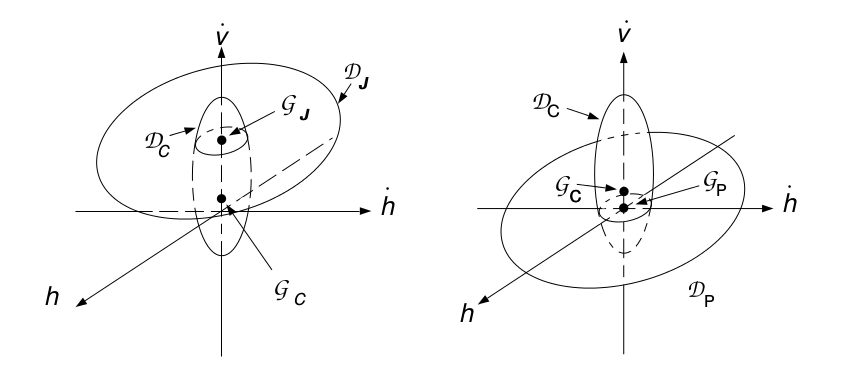
\includegraphics[width=90mm]{Koditschek1}
  \caption{Representation of the three different domains of the three controllers: juggle, catcher and palmer}
  \label{PhasePlane}
\end{figure}
\end{itemize}

\subsection*{Key points / Takeaways}
\begin{enumerate}
\item A \textit{pre-image}, in the paper of Lozano-Perez, can be seen as the set of all the points of the space that allow to reach a goal with a single discrete motion
\item The term \textit{back chaining} refers to process of splitting the trajectory from the goal back to the starting point in many \textit{pre-images} that corrispond to discrete movements.
\item It is shown that the vertical velocity $\dot{z}$ has little influence when compared to the general horizontal speed $\dot{h}$ (either $\dot{x}$ or $\dot{y}$).
\end{enumerate}
\subsection*{Weak points}
\subsection*{Ideas}
\begin{enumerate}
\item Extend the idea of \textit{self-manipulation}: what if we reverse the problem of locomotion and we look at it as a manipulation problem? It is like considering that the earth is moving and the robot is a fixed frame. The manipulation consists in this case of many impacts which keep the earth in the "controllable region". 
\item analyse a way to approach the control of \textbf{Discrete Events Systems}. In between two following events the system can thus be seen as an \textbf{autonomous system} (we cannot change the trajectory of the CoM between two events, what we can do is only to adjust the angular orientation and the position of the feet at the next impact).
\item From the manipulation point of view: we deal with the control of a DES when we have an obstacle which disconnects the workspace.
\end{enumerate}
\section{D.E. Koditschek - The Penn Jerboa: a platform for exploring parallel composition of templates - Koditschek}
Authors: D.E. Koditschek\\
Year: 2015
\subsection*{Summary}
\subsection*{Key points / Takeaways}
\subsection*{Weak points}
\subsection*{Ideas}

\section{D.E. Koditschek - Legged Self-manipulation}
Authors: D.E. Koditschek\\
Year: 2015
\subsection*{Summary}
\subsection*{Key points / Takeaways}
\subsection*{Weak points}
\subsection*{Ideas}

\section{Rao - Numerical Methods for Optimal Control \cite{Rao} \cite{Betts}}
Authors: Rao\\
Year: 2010
\subsection*{Summary}
We can distinguish between 	\textit{trajectory optimization} and \textit{optimal control} problems mainly involved in control problems. The first case the optimization variables are static parameters while in the second case they are functions. In both cases the goal is to optimize (minimize or maximise) an objective index (which is a function in the case of trajectory optimization and it is a functional in the case of optimal control).\\
In the category of optimal control we can distinguish the following typical problems to be solved:
\begin{enumerate}
\item Systems of nonlinear equations
\item Differential equations and integration of function
\begin{itemize}
\item Time-marching
\begin{itemize}
\item Multiple-step methods (implicit (such as Euler forward, Crank-Nicolson or explicit liek Euler backward))
\item Multiple-stage methods (\textbf{Runge-Kutta} ''discretization '' method)\\
In this method we divide the period of interest subintervals of duration h (the smaller is h the better will be the approximation). In this way the period is ''discretized''. The typical Runge-Kutta method is a fourth order method, meaning that the value of each stage is computed by means of 4 parameters. This method is very good \textit{locally} in that the approximation performance decrease faw away from the initial stage.
\end{itemize}
\item Collocation\\
\begin{itemize}
\item Gauss
\item Radau
\item Lobatto
\end{itemize}
This methods aim at approximating a function with a polynomial, the order of which is determined by the number of conditions we can impose. Each condition refers to a time instant. All the \textit{collocation conditions} make up together a system where they are rewritten in the form of \textit{defect conditions}. The solution of this system leads to a \textit{simultaneous} computation of all the parameters (as an opposite to the \textit{predictor-corrector} approach found in time-marching).
\begin{itemize}
\item Orthogonal collocation: in this method the collocation points are roots of special family of polynomials named \textit{orthogonal polynomials} (e.g Legendre polynomials and Chebyshev polynomials). When the points are chose in an orthogonal mater (such as in this method) then the approximation to a definite integral is much more precise than the normal collocation methods.
\end{itemize}
\end{itemize}
\item Nonlinear optimization / Nonlinear Programming (NLP)
\begin{itemize}
\item Gradient-based methods
\begin{itemize}
\item Sequential Quadratic Programming (SQP)
\item Interior-point (IP)
\item Barrier methods
\end{itemize}
\item Euristic methods (stochastics)
\begin{itemize}
\item Genetic algorithms: each genetic algorithm is made of the following components: encoding, fitness, selection, crossover and mutation
\item Simulated annealing
\item Particle swarm optimization (PSO)
\end{itemize}
\end{itemize}
\end{enumerate}
The first two points are instances of problems to be solved with \textbf{indirect methods} while the second and the third are to be solved with \textbf{direct methods}. The second point can be solved with both methods.\\
\begin{itemize}
\item indirect methods/transcription: 
\item direct methods/transcription (discretize then optimize):
\begin{itemize}
\item control parametrization method
\item state and control parametrization method (such as direct collocation)
\end{itemize}
\end{itemize}
\subsection*{Key points / Takeaways}
\subsection*{Weak points}
\subsection*{Ideas}

\section{Wang - Model-Based Position and Force Controller for a Hydraulic Legged Robot \cite{ChenWang}}
Authors: Guangrong Chen , Junzheng Wang, Shoukun Wang, Jiangbo Zhao, and Wei Shen\\
year: 2016
\subsection*{Summary}
The compliance controller is a mix of active and passive compliance. The \textbf{realized compliance} $Z_r$ is defined as the ratio between the applied force/torque $F(s)$ and the resulting position error $e(s) = x_0(s)-x(s)$. It is proved that the quantity $Z_r(s)$ can also be written as:
$$ Z_r(s)  = Z_d(s) \cdot G_p^{-1}(s) $$ where $Z_d(s)$ is the desired compliance and $G_p(s)$ is the inner closed-loop transfer function.\\
The compression of the passive spring $p_e(s)$ is just a bit of the total compression $p(s)$:
$$ p_e(s) = [1+Z_r^{-1}(s) \cdot Z_e(s)]^{-1} \cdot p(s)$$
As regards the stability we can say that the passive part of the system (the passive spring) is stable if the all system is stable and viceversa. In order for this property to hold in this system we need the term $[1+Z_r^{-1}(s) \cdot Z_e(s)]^{-1}$ to be stable. This is verified if $K_r \geq min(K_e, K_p)$ where $K_r$ is the realized impedance of the system, $K_e$ is the one of the passive spring (the environment) and $K_p$ is the one of the active part.
\subsection*{Key points/ Takeaways}
\begin{itemize}
\item two main conditions for a compliance controller to be stable: the inner c.l. transfer function must be stable and  $K_r \geq min(K_e, K_p)$ must hold true.
\item in the system described in this paper, a quadruped robot with passive springs in its legs we can define the total compliance as mix of active and passive one. The passive compliance term is a pure stiffness $K_e$, while the active term is composed of stiffness $K_r$ and damping $B_r$ (also named \textit{dissipation component}). The damping part is due to the friction of the hydraulic actuators.
\item The Baud-rate on a CANBUS device refers to the rate (speed) at which data is transmitted on the network. This is typically expressed in kilobits-per-second (kbps). In this case the CAN BUS baud-rate is 1000 kbps, cio\'e 1 Mbps (The baud-rate of a EtherCat can be up to 100 Mbps)
\item A method is proposed at page 4 to define the desired reference stiffness $K_d$ given the vicious friction (viscous friction) $B_r$ of the hydraulic actuators.
\item The compliance control sensibly reduces the peak in the impact force and the settling time is also considerably reduced.
\item The compliant behavior cannot be achieved by only active compliance control if the controller is not fast enough. The adjoint of a passive spring reduces the impact force peak and makes the impact duration longer, giving more time to the controller in order to react.
\item The Swing Leg Retraction (SLR), even if so far it was not assessed how to generate it, it does clearly reduce the impact forces
\item In the case of ideal stiff actuator we assume that the actuator can reach in one single sample the desired value. In this case the inner closed-loop transfer function and $G_p = I$ and the position error transfer function $E_p = 0$.
\end{itemize}
\subsection*{Weak Points}
\begin{itemize}
\item Shouldn't the title mention the world ''compliance''? e.g. ''mix of active and passive compliance''
\item Figure n. 2 is not explained at all
\item At line 52 page 2 right column two words are missing so the meaning of the whole sentence is not clear
\item It looks like the robot is equipped with a spring on the leg, so the final compliance is a mix of active and passive one. This should be stated more clearly in the intro
\item Figure 6: The letter P does not appear so it is not straighforward to read the image. Also F is not represented in the image whilst H is drawn twice so it might have two different meanings. Also the \textit{landing angle} $\alpha$ should be represented in this figure.
\item is it "vicious friction" or "viscous friction" (referred to the damping factor of the hydraulic actuators)?
\item How could they get the blue dotted curve in figure 11? Didi they have to lock the actuators to obtain it?
\item it should better be defined what a \textbf{passive system} is. A passive system in general is defined as a system where there is energy dissipation (such as the damping of spring-damper or such as the induction). In the considered system the dissipation is given by the term $B_r$ which represents the damping of the active spring.
\item the compliant behavior can be usually achieved in two ways: 
\begin{enumerate}
\item the force info is multiplied by the inverse of the desired impedance in order to compute the corresponding compression of the joints (this is called \textbf{admittance} control);
\item the compression $\Delta \theta$ and the joint velocity $\dot{\theta}$ are multiplied by a stiffness factor $P_{gain}$ and a damping factor $D_{gain}$ (this is referred to as \textbf{impedance} control)
\end{enumerate}
In both way the force info (or the compression and speed info) can either come from the end-effector only, or from each joint of the leg.
\end{itemize}
\subsection*{Ideas}

\section{Wang - A strategy for push recovery in quadruped robot based on reinforcement learning - 2015}
\section{Dynamic Torque Control of a Hydraulic Quadruped Robot \cite{SeminiFocchi}}
Authors: Thiago Boaventura, Claudio Semini, Jonas Buchli, Marco Frigerio, Michele Focchi, Darwin G. Caldwell\\
year: 2012
\subsection*{Summary}
Main features required to a quadruped robot controller:
\begin{itemize}
\item precise: able to perform accurate footholds placement
\item fast: able to produce fast movements
\item robust: needed against uncertainties and disturbancies
\item compliant: needed to withstand impacts and crashes
\end{itemize}
The \textbf{whole-body control} is a model-based controller which operates through an inversion of the dynamics, this can be seen as a \textbf{force/torque control}. The \textbf{position control} will still be present as a lower level control but will have low gains and thus have a little influence on the lower higher level.\\
When we talk about stability in the field of dynamic motions we had better refer to \textbf{limit-cicle stability}.
\subsection*{Key points / Takeaways}
\begin{itemize}
\item the controller can be described as a three-layer controller:
\begin{itemize}
\item The outer layer is a position control in the joint space
\item the middle layer is a force/torque controller
\item the inner layer is a position/speed control in the operational space and a pressure controller
\end{itemize}
All these quantities are linearized thanks to a feedback linearization which leads to a linearized input $v$, this is computed as a PID controller. This PID controller is also responsible for the compliance of the system: in order to keep safe the mechanical parts and the electronics from impacts the torque peaks are always kept at safe level underneath 160 Nm.
\item The robustness of the controller is not only achieved by means of robust controllers but also with robust hardware. The flow of the valves must have a large bandwith so that it can meet the requirements of different gaits.
\item An equation for force control for hydraulically actuated robots can be computed using the \textit{Bernoulli} equation (force equilibrium) \cite{ThiagoSemini}. 
\end{itemize}
\subsection*{Weak Points}
\subsection*{Ideas}

\section{Focchi, Semini et al. - Gain scheduling control for the hydraulic actuation of the HyQ robot leg}
Authors: B. Cunha, Thiago and Claudio, Semini and Emanuele, Guglielmino and Michele, Focchi and Darwin G., Caldwell\\
Year: 2010
\subsection*{Summary}
\subsection*{Key points / Takeaways}
\subsection*{Weak points}
\subsection*{Ideas}
\section{Focchi, Semini et al. - Robot Impedance Control and Passivity Analysis
with Inner Torque and Velocity Feedback Loops \cite{SeminiFocchi2}}
Authors: Michele Focchi\\
Year: 2014
\subsection*{Summary}
The interest of this paper is to identify the values of the parameters which yield a stable impedance in the system. In particular the focus is given to the HAA joint of HyQ.\\
The controller is a nested structure of three layers:
\begin{itemize}
\item inner positive feedback control loop (velocity compensation gain $\alpha$). Here the velocity is obtained through derivative of the angular join position which yields highly noisy signals, as a consequence also a filter needs to be introduced, parametrized by $N_{av}$, to smooth the signal.
\item torque loop (proportional feedback gain $\beta$)
\item outer impedance control (PD controller with $P_{gain}$ and $D_{gain}$)
\end{itemize}
Besides the 5 parameters mentioned above also the sampling time $t_s$ has got a high influence on the stability of the system.\\
The stability analysis is here carried out highlighting the \textbf{passivity} property of the system. Passivity is a conservative condition which states that given a passive system (such as an obstacle in the environment) the robot interaction with that system will be stable if it also behaves in a passive way. Passive springs are always passive in that they induce energy dissipation, but an active compliant system may be passive only under a proper analysis. In this paper it is shown that a \textbf{driving port impedance transfer function} $Z(s)$ will be positive only under the two following conditions:
\begin{enumerate}
\item $Z(s)$ has no pole with positive real part
\item the phase of $Z(s)$ lies between -90 and 90$\degree$
\end{enumerate}
\textit{\begin{figure}
  \centering
  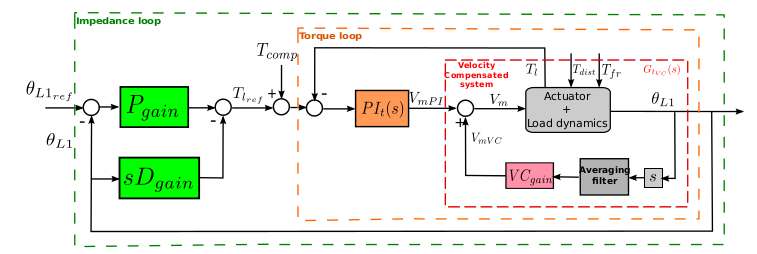
\includegraphics[width=120mm]{VelocityAndTorqueControl}
  \caption{Block diagram of the velocity compensated system with inner torque loop and outer impedance loop}
  \label{SpeedTorqueControl}
\end{figure}}
In the paper is also explained that, due to the derivative operator, the velocity compensator does not only influence the poles of the c.l.system (as the torque loop does), but it also affects the zeros of the system.
\subsection*{Key points / Takeaways}
\begin{itemize}
\item compliance might be limited by the bandwidth of inner control loops (such as torque control loops by instance). The \textbf{bandwidth} is defined as the frequency where the torque amplitude decreases by $-3$dB with respect to the reference system.
\item When we have a cascade of control loops it becomes fundamental to test the correct bandwidth of each loop. The bandwidth of the loop is connected to the time response, or more precisely, to the rise time in this way: $$ f(Hz) = \frac{1}{t_r(sec)}$$
In general in cascaded control loops we have that the \textbf{bandwidth} of the innermost loop as to be at least one order of magnitude faster than the outer loop. The higher the bandwidth (faster system) the better the tracking error, whilst the lower the bandwidth (for slow systems) the higher the \textbf{damping effect}. In robotic systems where we are interested in achieving compliant behaviors, the bandwidth must be tuned in order to find a trade-off between \textbf{tracking} error and impedance.\\
The bandwidth is directly affected by \textbf{sampling frequency} $T_s$ and \textbf{filtering} $N_{av}$ (number of samples to be filtered together): the lower the frequency of the system, the slower the system, the lower the bandwidth.\\
Usually in \textbf{nested control loops} the slowest frequency acts as a \textbf{bottleneck} for the whole system.
\item It is better to discretize the system and carry out the analysis in discrete domain because discretizing introduces many problems; for example a minimum phase system may become \textbf{non-minimum phase} when it is discretized.
\item Sampling time of the controller: $t_s=$ 1 ms
\item The compliance controller can be seen as nothing but the tracking of the joint angle with more or less high PD gains. High $P_{gain}$ and $D_{gain}$ will result in stiff behavior (low compliance) while low gains will result in high compliance.
\end{itemize}
\subsection*{Weak points}
\subsection*{Ideas}
\section{Gustavo A. Medrano-Cerda - Comparison of Various Active Impedance Control Approaches, Modeling, Implementation, Passivity, Stability and Trade-offs - 2012}
\subsection*{Summary}
Four main controllers have been here compared, all of them have in common the outer control loop based on torque feedback. These controllers are targeted at SEA (Series Elastic Actuators) where each motor is coupled with a elastic and damping factor. The Impedance control (IC) is achieved with a torque feedback:\\ "on motor side": $ \tau_d = \tau_c + K (\theta_{ref}-\theta_{mH}) - D(\dot{\theta}_{mH})$\\ or on the "link side: $ \tau_d = \tau_c + K (\theta_{ref}-\theta_{L}) - D(\dot{\theta}_{L})$\\
IC control can either be based on \textbf{motor side} or \textbf{link side}, thus all of the controllers shown below can have two possible versions. The motor side consists in supplying as a feedback the motor angles $\theta_m$ while the link side consists in supplying the link states $\theta_L$. These two states might differ mainly because of the elasticity of the links. The following controllers differ from the inner loop and the type of reference signal that the outer IC loop provides to the inner controller:
\begin{itemize}
\item ICT = Impedance control with explicit torque loop (and inner torque PID loop)
\item ICP = IC torque control with inner position PID control (damping gain D as small as possible)
\item ICVM = outer torque loop and inner velocity PI gain (motor side). This method could be used on HyQ (note that the term $\frac{1}{D}$ requires the damping gain D to be always quite big, which is the case for HyQ). The advantage of using the inner velocity-based PI controller is that passivity is granted also for high values of systems stiffness (which is not true for the torque-based PID);
\item ICVL = outer torque loop and inner velocity PI gain (link side);
\end{itemize}
\subsection*{Take aways}
\begin{itemize}
\item In the design of nested control loops it's not always sufficient to design the inner loop (of whichever kind, e.g. PID) with the highest bandwidth possible (chiefly when we deal with discrete systems). It was here shown that the outer \textbf{impedance control} loop (on \textbf{motor or link side}) might not be stable even for very high bandwidth of the inner loop. 
\item It is sometimes interesting to check the bandwidth not only of the overall controller but also of the innermost PID loop. The table below (figure \ref{ICperformance}) provides some performance of the bandwidth for different impedance controllers (ICT, ICP and ICV).\begin{figure}[h!]
  \centering
  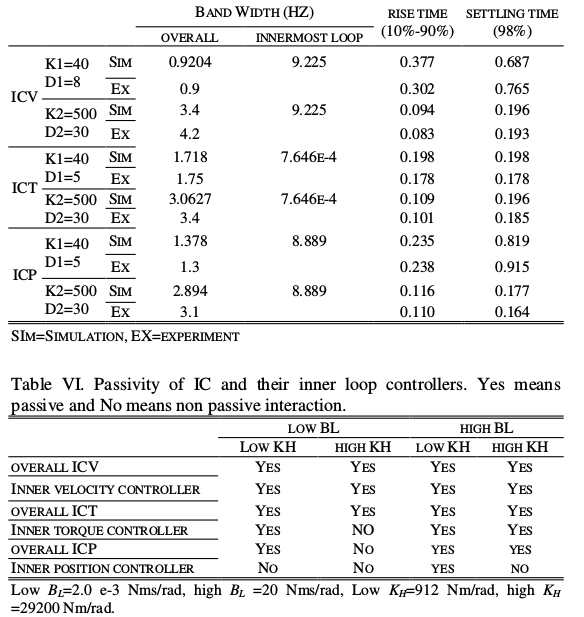
\includegraphics[width=120mm]{PassivityOfICcontrollers}
  \caption{Performance of ICT, ICP and ICV with respect to passivity for low and high stiffness and damping gains}
  \label{ICperformance}
\end{figure}
The bandwidth of the innermost PID loop is of importance when we have the inner PID loop running on the DSP (Digital Signal Processing) unit and we have the outer loop (impedance control) running on a centralized CPU. In the case the communication fails then the actuator will be left with the inner PID loop only. For this reason the higher the bandwidth of the inner loop the more robust is the system again communication failures.
\end{itemize}

\section{M. Diehl - Fast direct multiple shooting algorithms for optimal robot control}
\section{M. Diehl, S. Gros - Real Time MHE and MPC for a large scale mechatronic application - 2015}
\section{Betts - Practical methods for optimal control and estimation using Nonlinear programming \cite{betts2010practical}}
This stuff is very cool!
\section{K. Hauser - Motion Planning for legged and humanoid robots \cite{Hauser2008}}
year: 2008
\subsection*{Summary}
The author defines the existence of different \textit{modes} $\sigma$ which belong to the same family $\Sigma$. The dimension of $\Sigma$, $dim(\Sigma)$, is lower than the dimension of the configuration space $Q$. All the modes of the same family are non-intersecting each other, meaning that if the robot is moving on a given trajectory $q$ which is on the mode $\sigma_1$ and wants to move to the mode $\sigma_2$ (of the same family $\Sigma$), it will have to go through another family $F$ which interesects the family $\Sigma$.
\subsection*{Key points / Takeaways}
\begin{itemize}
\item PRM = Probabilistic Road Map
\item MMPRM = Multi Modal Probabilistic Road Map
\item family = foliation
\item mode = leaves
\item In legged locomotion a \textbf{mode} $\sigma \in \Sigma$ is a fixed set of footfalls. So $\sigma$ stands for \textit{stance} and $Q_{\sigma}$ is the configuration space that can be reached by all the robots joints when the given stance $\sigma$ is fixed. In general a mode $\sigma$ defines a \textit{feasible space} $F_{\sigma}$ which is the set of configurations that satisfy the mode-specific constraints. Namely $F_{\sigma}$ is a subset of $Q$ (the configuration space of $q$), limited by the \textit{dimensionality reducing constraints} and by the \textit{volume reducing constraints}
\begin{figure}[h]
  \centering
  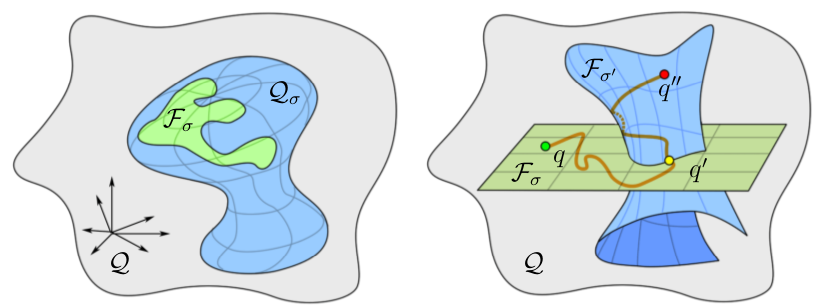
\includegraphics[width=120mm]{FamilyModes}
  \caption{Family modes}
  \label{OptimizationDiehl}
\end{figure}
\end{itemize}
\subsection*{Weak points}
\begin{itemize}
\item The author distinguishes between \textit{volume reducing constraints} and \textit{dimensionality reducing contraints}. And how can we classify the nonholonomic contraints then?
\end{itemize}

\subsection*{ideas}
\section{K. Hauser, O. Ramon - Generalization of the Capture Point to Nonlinear Center of Mass and Uneven Terrain \cite{RamonHauser2015}}
Year: 2015
\subsection*{Summary}
This paper generalizes the concept of Capture Point as we know it based on a LIP model on a flat terrain. The new model is a Nonlinear Inverted Pendulum, meaning that the height of the CoM is no more constrained to be constant but it can be a steep lin or a parabola. In the mean time also uneven terrains are considered, when characterized by a polygonal shape.
\subsection*{Key points / Takeaways}
See the Journal Club of 2016 on this paper.
\subsection*{Weak points}
\subsection*{Ideas}e or a parabola. In the mean time also uneven terrains are considered, when characterized by a polygonal shape.
\subsection*{Key points / Takeaways}
See the Journal Club of 2016 on this paper.
\subsection*{Weak points}
\subsection*{Ideas}
\begin{itemize}
\item extend to non-zero momentum case;
\item extend to more complex environments;
\item extend to more complex CoM trajectories;
\end{itemize}

\section{Boyd - Introduction to Linear Dynamical Systems}
\section{A. Bemporad - Model Predictive Control Course}
\section{A. Hof - The eXtrapolated Center of Mass concepts suggests a simple control of balance in walking \cite{AHof}}
\subsection*{Summary}
The phase diagram given in the paper is useful in order to show that the equilibrium point (when the CoM is exactly above the CoP) is an unstable equilibrium in the sense that a small disturbance will make the state change to another configuration.\\
The Capture Point (or XCoM) can be seen as the  
\subsection*{Key points/ takeaways}
\begin{enumerate}
	\item property 1: A sufficient condition for stability of the CoM trajectory is that the Xcom trajectory is stable (read: does not diverge too much compared to step length)
	\item property 2: At any point the tangent to the trajectory of the Xcom runs through the CoP.
\end{enumerate}
\subsection*{Weak points}
\section{P. Abbeel - Apprenticeship Learning and Reinforcement learning with application to robotic control - 2008}
\section{T. De Boer, J.Pratt - Thesis Ch.4 - Foot Placement Control: step location and step time as a function of the desired walking gait}
\subsection*{Summary}

This chapter it is proved how the \textbf{Dynamic Foot Placement algorithm} outperforms the \textbf{constant offset algorithm} in terms of number of steps needed to reach the desired cyclic gait and in terms of viable initial conditions. The former is not done by optimal control but it is rather carried out in closed-form solution thanks to the consideration that the foot placement problem has got a number of decision variables dependent from the number of steps which we want to perform. The algorithm asses first the 0-steps problem in which the only decision variable is the time duration $t_0$ of the step. In this case the problem is over-constrained because there are four equations and only one decision variable.\\
If the initial condition do not fit well the desired gait cycle then the 1-step strategy is adopted. In this case the problem is fully-constrained because we have four equations and four variables ($t_0, t_1$ and $S_0$)\\
In the case that this strategy does not respect the torque limits (imposed on time) or the maximum step length constraint then the 2-steps strategy is implemented (which is under-constrained).

\subsection*{Take aways}
\begin{enumerate}
\item the Dynamic Foot Placement algorithm, given a desired cyclic gait (given in form of initial guess for the CoP position and step time), provides the suitable foothold and step time for the next step. It is not bound to a particular planner, so it can be used by some high-level planner to determine the necessary footholds.
\item The performances of the foot placement planner are counted in terms of the \textbf{number of steps needed} to reach the desired gait limit cycle.
\item The problem is solved with closed-form expressions rather than using optimal control (which is not suitable for real time applications)
\item this approach does not keep into account the mechanical work of the system and uses the 3d-LIP model which is very simplistic

\end{enumerate}
\subsection*{Ideas}

\begin{itemize}
\item In this paper it is assumed that a step has no instantaneous effect
on the velocity of the point mass... what about considering it instead?? Every impact could be considered as a loss of energy dependent on the compliance of the robot!!!

\item what about computing a \textit{capture speed} rather than a \textit{capture point}? Obviously when the speed is null the capture speed should reduce to the capture point.
\end{itemize}
\section{Todorov - Infinite-Horizon Model Predictive Control for Periodic Tasks with Contacts - 2011}
\section{Englsberger, Ott - Biologically inspired deadbeat control for running on 3d stepping stones - 2015}
\section{Englsberger, Ott - Biologically inspired deadbeat controller for bipedal running in 3D - 2015}
\section{Nakanishi, Mistri, Schaal - Operational Space Control: A theorical and Empirical Comparison - 2005}

\subsection*{Summary}
Operational Space controllers can be subdivided in mainly 8 types:
\begin{itemize}
\item 
\end{itemize}
\subsection*{Take aways}
\section{Fukuoka - A simple rule for quadrupedal gait generation determined by leg loading feedback: a modeling study - 2015}

\subsection*{Summary}

 "It has been posited that in well-predicted movements, CPG-generated phase durations and muscle forces closely match those required by the evolving biomechanical events, minimizing the sensory corrections required. The term ‘‘neuromechanical tuning’’ has been coined to describe this process"
\section{Fukuoka - Adaptive Dynamic Walking of a Quadruped Robot on Irregular Terrain Based on Biological Concepts - 2003}
\section{Siciliano, Khatib - Handbook of Robotics, ch. 7, Force Control - 2008}
\subsection*{Impedance Control}
\subsection*{Admittance Control}
\subsubsection*{Difference between impedance and admittance control}

\begin{itemize}
\item \textit{impedance control}: when, given a certain displacement, a corresponding reaction force is imposed. The impedance controller feedback is an acceleration in the task space that, with inverse dynamics, can be translated into a force in the joint space (figure \ref{ImpContr}).
\item \textit{admittance control}: as opposite to impedance control here, given a certain interaction force, a corresponding motion (position and velocity) is imposed (figure \ref{admitContr}). This can be done be decoupling the impedance controller into two parts, one in charge of tracking the reference motion and on in charge of a compliant frame. This compliant frame coincides with the desired frame when there is no interaction. In presence of interaction instead the motion controller will rigidly track the reference given by the compliant frame.
\item \textit{damping control}
\item \textit{stiffness control}
\end{itemize}

\begin{figure}[h]
  \centering
  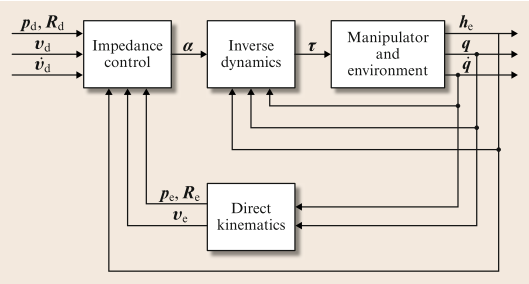
\includegraphics[width=100mm]{ImpedanceControl}
  \caption{Impedance control}
  \label{ImpContr}
\end{figure}
\begin{figure}[h]
  \centering
  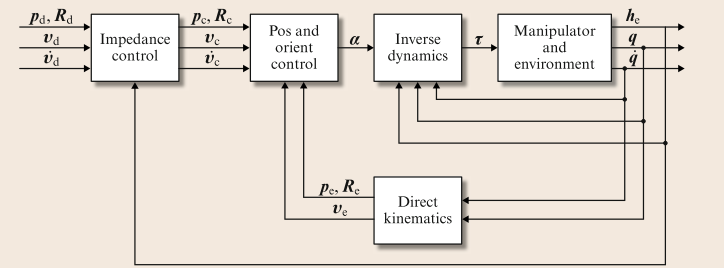
\includegraphics[width=100mm]{AdmittanceControl}
  \caption{Admittance control}
  \label{admitContr}
\end{figure}
\section{Maes - Steady locomotion in dogs: temporal and associated spatial coordination patterns and the effect of speed - 2007}

\subsection*{Summary}
\subsection*{Take aways}

\begin{enumerate}
\item The duty factor of the front legs in dogs is usually not the same of hind legs. At low speeds the the front legs need to support the weight of the body (in dogs more than 60\% of the total mass weights on the front legs) so the duty factor ($T_{st}/T$) of front legs is higher than the one of hind legs. As an opposite, at high speeds the propellant role of hindlimbs takes over and therefore the duty factor of the hindlimbs increases and becomes larger than the one of front legs.
\end{enumerate}
\section{Walter, Carrier - Ground force applied by galloping dogs - 2006}
\section{Walter, Carrier - Rapid acceleration in dogs: ground reaction forces and posture dynamics - 2009}

\subsection*{Summary}

\begin{multicols}{2}
[
Steady-state locomotion compared to rapid accelerations:
]
\textbf{Steady-state locomotion:}
\begin{itemize}
\item Front legs support 56-64 \% of the body weight
\item On humans it was observed that also legs stiffness is correlated to maximum speed, besides power and strenght. For rapid accelerations instead stiffness plays no role.
\item Duty factors are much lower (shorter stance phase) even for ''long-stance'' gaits such as trot and pace
\end{itemize}
\columnbreak

\textbf{Rapid accelerations:}
\begin{itemize}
\item Front legs support 43 \% of the body weight
\item Limbs are more retracted and flexed in order to use all the range of motion. The propulsive force is thus produced for a larger range of motion.
\item Trunk experiences greater pitching movement
\item Much higher force peaks (2 or 3 times higher)
\item Ground forces are entirely propulsive (almost no braking in the first steps).
\item Half-bound was the preferred gait
\item vertical forces in fore limbs increase step by step together with speed and stance time decreases.
\item angular excursion of about $28\degree$ which is 38 \% more than the excursion of steady-state
\item the \textit{head-end down} configuration (positive pitch) helps to lower down the CoM and thus bring the GRF alligned to the CoM.
\item The optimal swing time is simply the shortest time required to reposition the legs (internal work). \textbf{The shorter is the swing time, the better.}
\end{itemize}

\end{multicols}

\begin{figure}[h]
  \centering
  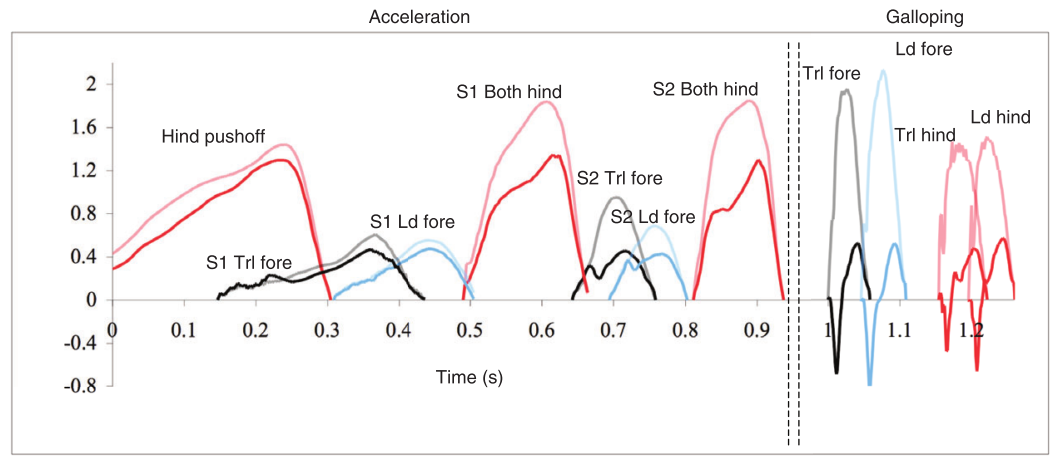
\includegraphics[width=150mm]{figs/RapidAccelerations}
  \caption{Rapid accelerations on dogs: this plots refer to a \textbf{half-bounding gait (hind legs move together while front legs are sequential: leading+trailing leg)}}
  \label{RapAcc}
\end{figure}
\subsection*{Experimental observations}
\begin{multicols}{3}
\textbf{Front legs:}
\begin{enumerate}
\item No braking forces were applied with the forelimbs during the first two accelerating strides.
\item stance time decreases when speed increases
\item vertical ground force of fore limbs increases with speed.
\end{enumerate}
\columnbreak

\textbf{Hind legs:}
\begin{enumerate}
\item The highest vertical ground forces are measured in the second step, as they decrease when the gait goes to steady state.
\item stance time decreases when speed increases
\item The orientation of the hind ground forces is strikingly constant
\item greater force is produced in the last part of the stance when joints are extending more rapidly
\end{enumerate}
\columnbreak

\textbf{Pitch:}
\begin{enumerate}
\item To avoid net pitching of the torso during locomotion, a quadruped’s net ground reaction force vector must pass through its center of mass.
\item The unavoidable pitching motion at start is slowly converted into linear speed when the dog reaches the steady state speed.
\end{enumerate}



\end{multicols}

\section{Hudson - High speed galloping in the cheetah (Acinonyx jubatus) and the racing greyhound (Canis familiaris): spatio-temporal and kinetic characteristics - 2012}


\subsection*{Summary}

\begin{itemize}
\item both cheetah and greyhounds use rotary gallop at fast speeds ($>14 m s^{-1}$). It is still unclear why the rotary gallop is preferred to transverse gallop, probably because of the reduced momentum losses during stance. The rotary gallop may become transverse gallop during abrupt direction changes (front legs are used to give yaw direction). 

\item There is a time-constant (short) aerial phase between the \textit{leading hind} leg and the \textit{trailing front} leg which is not dependent from speed. There is then another aerial phase which increases with speed and takes place between the \textit{trailing front} leg and the \textit{leading hind} leg. During this aerial phase the cheetah/greyhound extends his trunk. This phase gets longer with increased speed and it thus appears only at higher speeds. At slow speeds therefore the stance of the \textit{leading hind leg} and the stance of the \textit{trailing front leg} can be almost coincident, in this case this gate is named \textbf{canter} (or \textbf{three-beat transverse gallop}).

\item Cheetahs use significantly shorter duty factors than greyhounds (i.e. cheetahs have shorter stance times).  Cheetahs swing time slightly decreases with speed while greyhounds swing time slightly increases. In general we can say that the swing time keeps constant with speed (between $200$ and $300 ms$)

\item cheetahs increase the peak of the \textbf{hind legs} contact forces with speed (to compensate the decrease of the stance time and keep the total impulse constant) while the \textbf{front legs} contact forces do not increase more than $900N$, probably because of muscles limits.

\item the maximum speed is limited by a mix of:
\begin{enumerate}
\item swing time limit
\item ground speed matching
\item muscular power available for external work
\item peak force that the limbs can withstand
\item maintaining stability
\item mental motivation of the animal 
\end{enumerate}

\item the body weight is not symmetrically distributed on the four legs. At steady state 56 \% of the weight is on the front legs, 27 \% is charged on the \textbf{trailing hind leg} and 17\% on the \textbf{leading hind leg}. During accelerations instead more than 50\% of the weight is supported by the hind legs.
\end{itemize}
\section{Hobbelen - A disturbance rejection measure for limit cycle walkers: the gait sensitivity norm - 2007}

\subsection*{Summary}
The gait sensitivity norm is a stability measure which evaluates the effect of a given disturbance $e$ on a given cyclic quantity $g$. $g$ can be a scalar or a vector containing the some state of a limit cycle walker, like its speed or the joint angles. For simplicity in the paper only one scalar $T^*$ is chosen, which represents the nominal $cycle time$ of the limit cycle walker.\\
The author proves that, in the easiest model of a walker (compass model), the cycle time $T^*$ and the robustness of the gait (i.e. not falling) are tightly connected. A variation of the actual cycle time  $T$ (which happens when there is some height variation in the ground) will necessarily make the robot fall forward (step-down case) or backward (step-up case). Therefore the cycle time $T$ is a good state for $g$.\\
Definition of \textbf{Gait Sensitivity Norm}:
$$  ||\frac{\partial \mathbf{g}}{\partial \mathbf{e}}||_2 = \frac{1}{|e_0|} \sqrt{\sum_{i=1}^q \sum_{k=0}^\infty (\mathbf{g}_k(i) - \mathbf{g^*}(i))^2}$$
where $k$ is the number of steps after that the disturbance $e_0$ has been applied. $q$ is the number of elements of the vector $\mathbf{g}$.\\
The authors prove that the gait sensitivity norm approximates the Basin of Attraction \textbf{BoA} (which is the real set of initial states which lead to a stable limit cycle gait) much better than other measures such as:
\begin{itemize}
\item \textbf{largest allowable deterministic disturbance} which can be applied (a height variation or a push on the hip for example);
\item \textbf{Largest Floquet multiplier}.
\end{itemize}
The gait sensitivity norm can be computed very quickly using therefore experimental data coming from simulations.\\
An analytic form of the gait sensitivity norm can also be computed by computing a fixed point $\mathbf{v}$ performing a Newthon-Raphson search as done by McGeer [\textbf{Passive Dynamic Walker}] and then linearizing. 
$$  ||\frac{\partial \mathbf{g}}{\partial \mathbf{e}}||_2 = \frac{1}{|e_0|} \sqrt{trace(D^T D) + \sum_{k=0}^\infty trace(B^T (A^T)^k C^T C A^k B)} $$
where $A, B, C$ and $D$ are the sensitivity matrices of the system:
$$ \Delta \mathbf{v}_{n+1} = A \Delta \mathbf{v}_n +B \mathbf{e}_n$$
$$ \Delta \mathbf{g}_{n+1} = C \Delta \mathbf{v}_n +D \mathbf{e}_n$$
\section{Bertram, Guntman - Motions of the running horse and cheetah revisited: fundamental mechanics of the transverse and rotary gallop - 2009}

\begin{figure}[h]
  \centering
  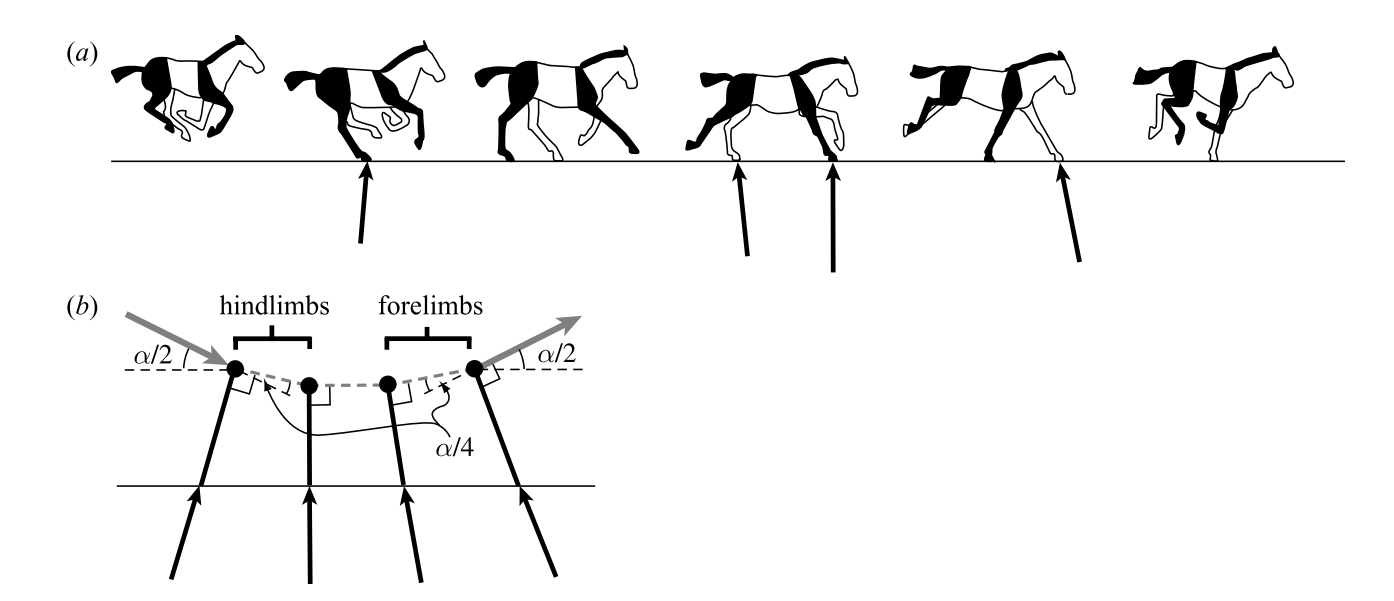
\includegraphics[width=140mm]{figs/HorseGallop}
  \caption{Horse transverse gallop}
  \label{horse}
\end{figure}

\begin{figure}[h]
  \centering
  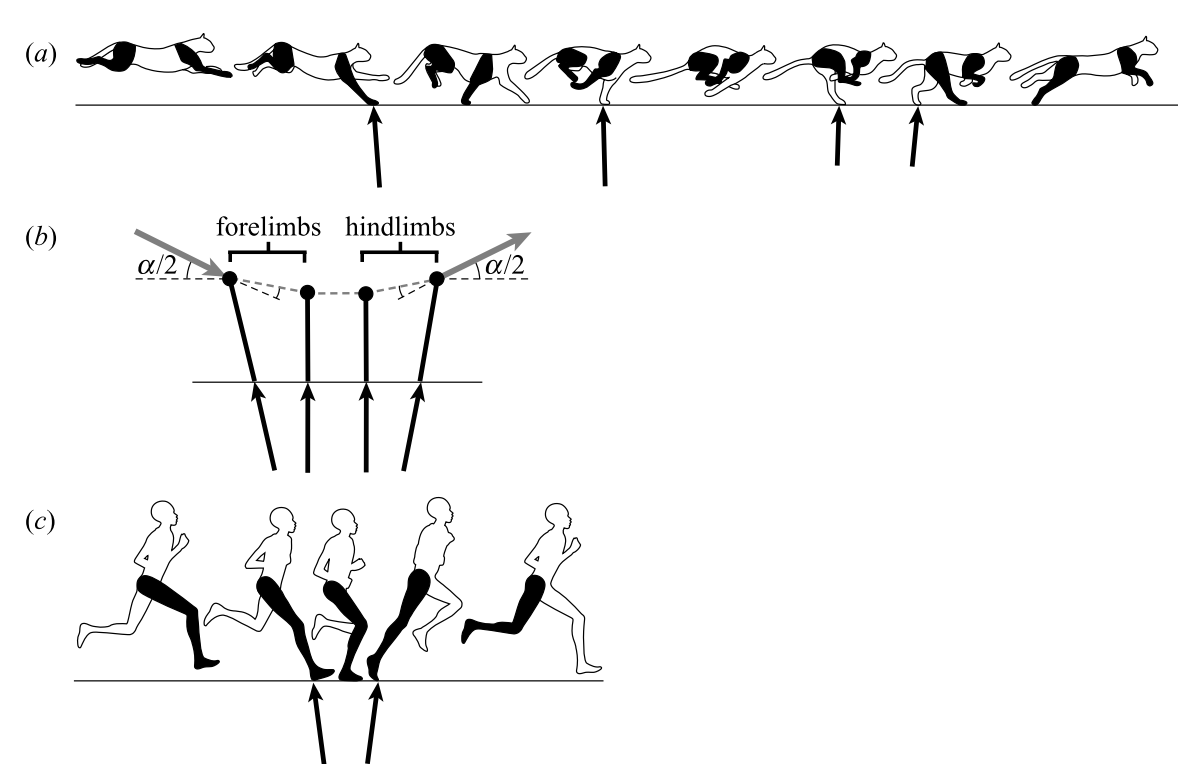
\includegraphics[width=140mm]{figs/CheetahGallop}
  \caption{Cheetah rotary gallop}
  \label{cheetah}
\end{figure}

\subsection*{Summary}
\begin{itemize}
\item The sequence of four-beat gallop (either rotary or transverse) helps the animal distribute over four impacts the direction change of an angle $\alpha$. Each contact contributes with a direction change of $\alpha/4$, regardless which leg is actually performing each impact.

\item The all purpose of a galloping gait is to \textbf{redirect the trajectory of the CoM} from forward-downward (at the end of the aerial phase) to an upward-forward (at the end of the cycle) direction. Rather than the \textit{rotary or transverse gallop} one should pay more attention to which limb initiate first the CoM trajectory transition. As a matter of fact when the forelimbs initiate this change of direction the resulting gait is a cheetah-like rotary (or lateral) gallop while when the hind legs initiate this result in a transverse (or diagonal) gallop. \textbf{The lateral coordination is of smaller importance} since both gaits can be realized even with perfectly parallel hind and front legs (\textbf{half-bound} if only the hind legs are coordinated and \textbf{bound} if also the front limbs are coordinated).

\item We can see in figure \ref{horse} (b) and \ref{cheetah} (b) that both transverse and rotary gallop achieve the same redirection of the CoM trajectory dury the cycle but the leg sequence and the direction of the ground reaction forces are completely different. \textbf{The GRF of the rotary gallop is more similar to the GRFs observed on human gaits}. Therefore the gallop \textbf{achieves in four impacts the same spring like behavior obtained by humans in one single stance.}

\item In order achieve the same kinetic energy at the  start and at the end of the cycle there are two methods: (a) storing the energy and give it back at the end of the stance (spring-like model); (b) reducing the energy loss in the first place (\textbf{pseudo-elastic model}). The latter model is based on the observation that: \textbf{a single limb that changes length in a manner that minimizes impulse along its axis could have much the same effect as a large number of limbs, each of a different length, acting in a sequence}.\\
The gallop works as a combination of spring-like and pseudo-elastic model.

\end{itemize}



\bibliographystyle{unsrt}
\bibliography{mybib.bib}
\end{document}